
\begin{frame}{FSMD : architecture contrôleur-chemin de données}
  \begin{alertblock}{FSMD \textit{explicite}}
    \begin{itemize}
      \item Finite State Machine + Datapath : microarchitecture dédiée à un algorithme.
    \end{itemize}
  \end{alertblock}
  \begin{columns}
    \begin{column}{0.5\textwidth}
      \begin{itemize}
        \item \textbf{Décomposition} explicite contrôle-données :
        \begin{itemize}
          \item Rôle de la \textbf{FSM} :
          \begin{itemize}
            \item Observation d'un signal de \textbf{démarrage}.
            \item \textbf{Séquencement} des calculs.
            \item Observation des \textbf{status} au cours des calculs et \textbf{prises de décision}.
            \item Activation des \textbf{contrôles}.
            \item Emission d'un signal de \textbf{terminaison}.
          \end{itemize}
          \item Rôle du \textbf{Datapath} :
          \begin{itemize}
            \item Réception des données externes
            \item Stockage des données internes
            \item Calculs (souvent parallèles)
            \item Production des sorties
          \end{itemize}
        \end{itemize}
        \item Il s'agit d'une structure \textbf{générique}.
      \end{itemize}
    \end{column}
    \begin{column}{0.5\textwidth}
      \begin{center}
        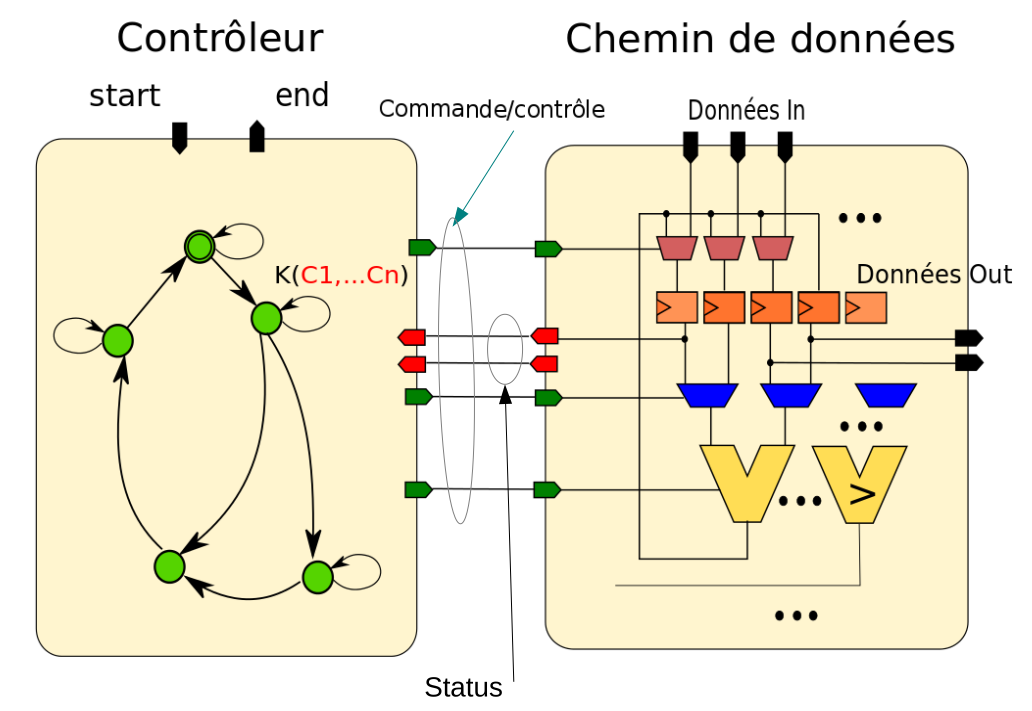
\includegraphics[scale=0.2]{./images/fsmd_0}
      \end{center}
    \end{column}
  \end{columns}
\end{frame}

\begin{frame}{FSMD : généricité du \texttt{datapath}}
  \begin{columns}
    \begin{column}{0.45\textwidth}
      \begin{itemize}
        \item Quatre étages ou \textit{couches} internes :
        \begin{enumerate}
          \item Couche de routage (mux):
          \begin{itemize}
            \item Acheminement des données aux registres
          \end{itemize}
          \item Couche de registres :
          \begin{itemize}
            \item Stockage des variables
          \end{itemize}
          \item Couche de routage (mux):
          \begin{itemize}
            \item Acheminement des données aux opérateurs.
          \end{itemize}
          \item Couche d'opérateurs :
          \begin{itemize}
            \item calculs arithmétiques et logiques.
          \end{itemize}

        \end{enumerate}
      \item Notez les possibilités importantes de \textbf{parallélisme de calculs} simultanés.
      \end{itemize}
    \end{column}
    \begin{column}{0.55\textwidth}
      \begin{center}
        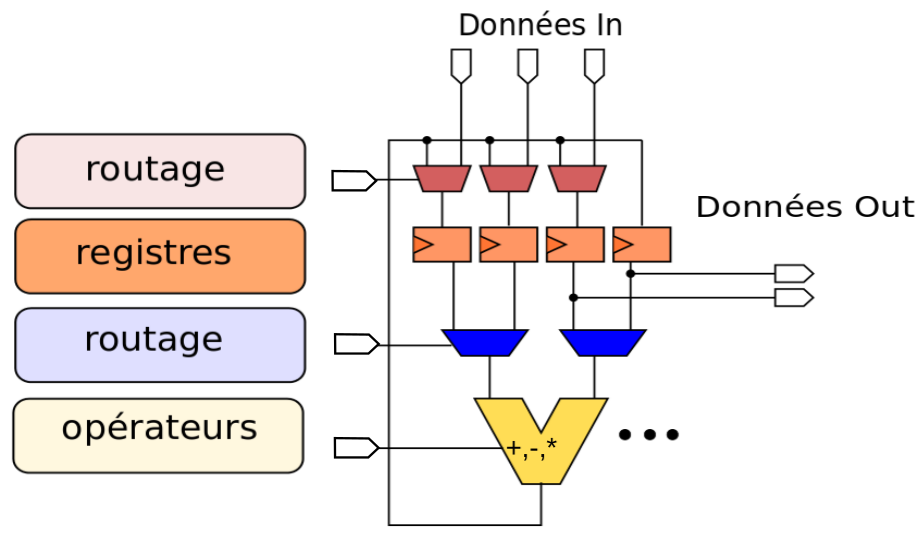
\includegraphics[scale=0.35]{./images/datapath_1}
      \end{center}
    \end{column}
  \end{columns}
\end{frame}

\begin{frame}{Algorithme du PGCD d'Euclide (par soustractions)}
  \textbf{Rappel : } Environ \textbf{300 av. J.-C.}
    \begin{columns}[T]

        % --- COLONNE 1 : L'ALGORITHME ---
        \begin{column}{0.55\textwidth}
            \begin{block}{Pseudo-code}
                \begin{algorithmic}[1]
                    \State $reg_a \gets \text{read}(data)$
                    \State $reg_b \gets \text{read}(data)$
                    \While{$reg_a \neq reg_b$}
                        \If{$reg_a > reg_b$}
                            \State $reg_a \gets reg_a - reg_b$
                        \Else
                            \State $reg_b \gets reg_b - reg_a$
                        \EndIf
                    \EndWhile
                    \State \Return $reg_a$
                \end{algorithmic}
            \end{block}

        \end{column}

        % --- COLONNE 2 : EXEMPLE CONCRET ---
        \begin{column}{0.40\textwidth}
            \begin{block}{Exemple : PGCD(48, 18)}
                \small
                \begin{center}
                    \begin{tabular}{c|c|c}
                        \textbf{Étape} & \textbf{reg\_a} & \textbf{reg\_b} \\
                        \hline
                        Init & 48 & 18 \\
                        1 & 30 & 18 \\
                        2 & 12 & 18 \\
                        3 & 12 & 6 \\
                        4 & 6 & 6 \\
                        \hline
                        \textbf{Fin} & \multicolumn{2}{c}{\textbf{Retourne 6}}
                    \end{tabular}
                \end{center}
                \vspace{0.2cm}
                \footnotesize \textit{À la fin de la boucle, les registres sont égaux.}
            \end{block}
        \end{column}

    \end{columns}


\end{frame}

\begin{frame}{FSMD : exemple \texttt{GCD} (Euclide)}
  \begin{center}
    \fbox{\textbf{Datapath} : quels calculs ? quels stockage ? quels routages ?}
  \end{center}
  \begin{columns}
    \begin{column}{0.40\textwidth}
      \begin{block}{Pseudo-code}
          \begin{algorithmic}[1]
              \State $reg_a \gets \text{read}(data)$
              \State $reg_b \gets \text{read}(data)$
              \While{$reg_a \neq reg_b$}
                  \If{$reg_a > reg_b$}
                      \State $reg_a \gets reg_a - reg_b$
                  \Else
                      \State $reg_b \gets reg_b - reg_a$
                  \EndIf
              \EndWhile
              \State \Return $reg_a$
          \end{algorithmic}
      \end{block}
    \end{column}
    \begin{column}{0.50\textwidth}
      \begin{center}
        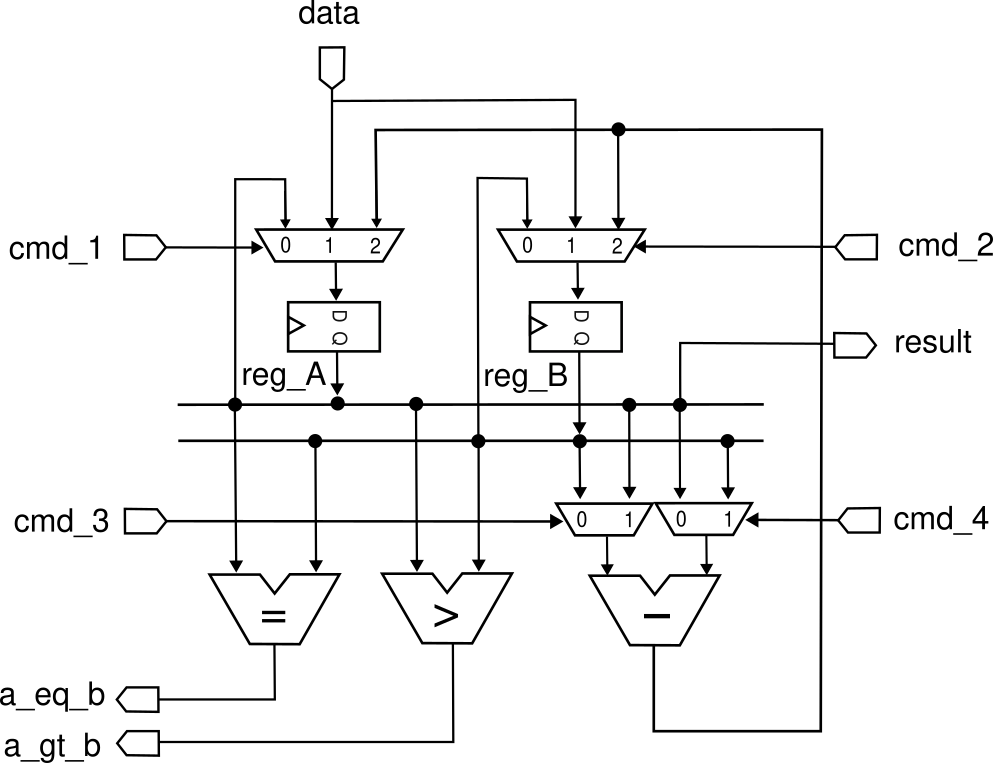
\includegraphics[scale=0.28]{./images/gcd_0}
      \end{center}
    \end{column}
  \end{columns}
\end{frame}

\begin{frame}{FSMD : exemple \texttt{GCD} (Euclide)}
  \begin{center}
    \fbox{\textbf{Contrôleur (FSM)} : Quelle séquence ? Quelles prises de décision ? Quelles actions sur le \textit{datapath} ?}
  \end{center}
  \begin{columns}
    \begin{column}{0.40\textwidth}
      \begin{block}{Pseudo-code}
          \begin{algorithmic}[1]
              \State $reg_a \gets \text{read}(data)$
              \State $reg_b \gets \text{read}(data)$
              \While{$reg_a \neq reg_b$}
                  \If{$reg_a > reg_b$}
                      \State $reg_a \gets reg_a - reg_b$
                  \Else
                      \State $reg_b \gets reg_b - reg_a$
                  \EndIf
              \EndWhile
              \State \Return $reg_a$
          \end{algorithmic}
      \end{block}
    \end{column}
    \begin{column}{0.50\textwidth}
      \begin{center}
        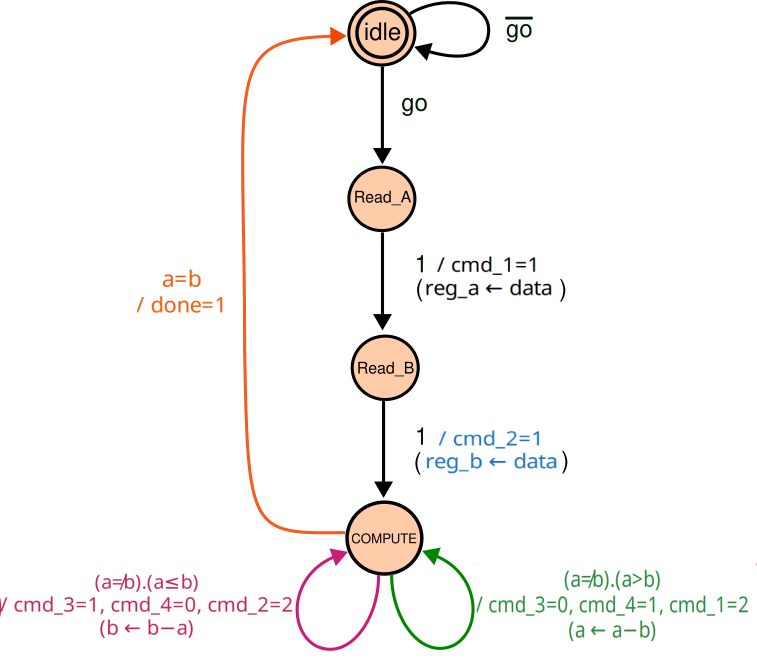
\includegraphics[scale=0.32]{./images/gcd_fsm}
      \end{center}
    \end{column}
  \end{columns}
\end{frame}

\begin{frame}{FSMD \texttt{GCD} : Assemblage FSMD}
  \begin{columns}
    \begin{column}{0.40\textwidth}
      \begin{center}
        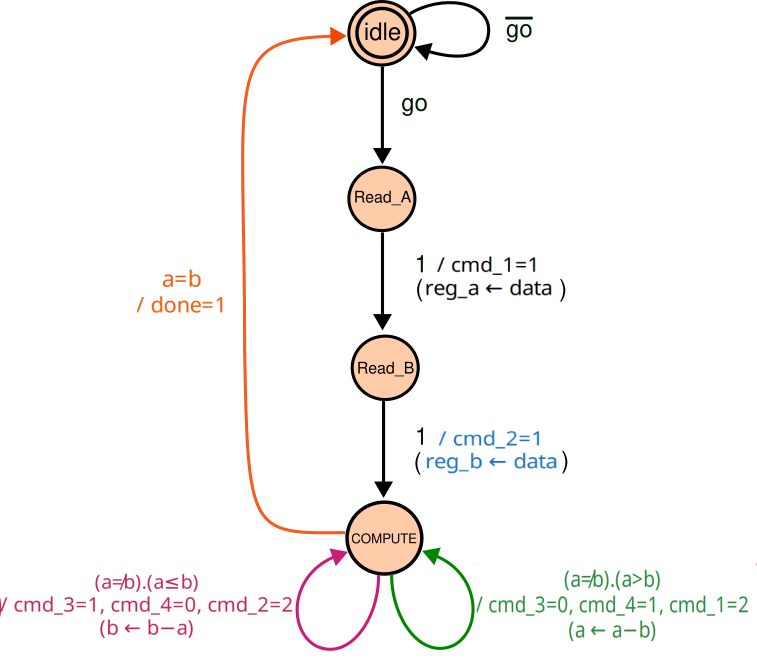
\includegraphics[scale=0.32]{./images/gcd_fsm}
      \end{center}
    \end{column}
    \begin{column}{0.50\textwidth}
      \begin{center}
        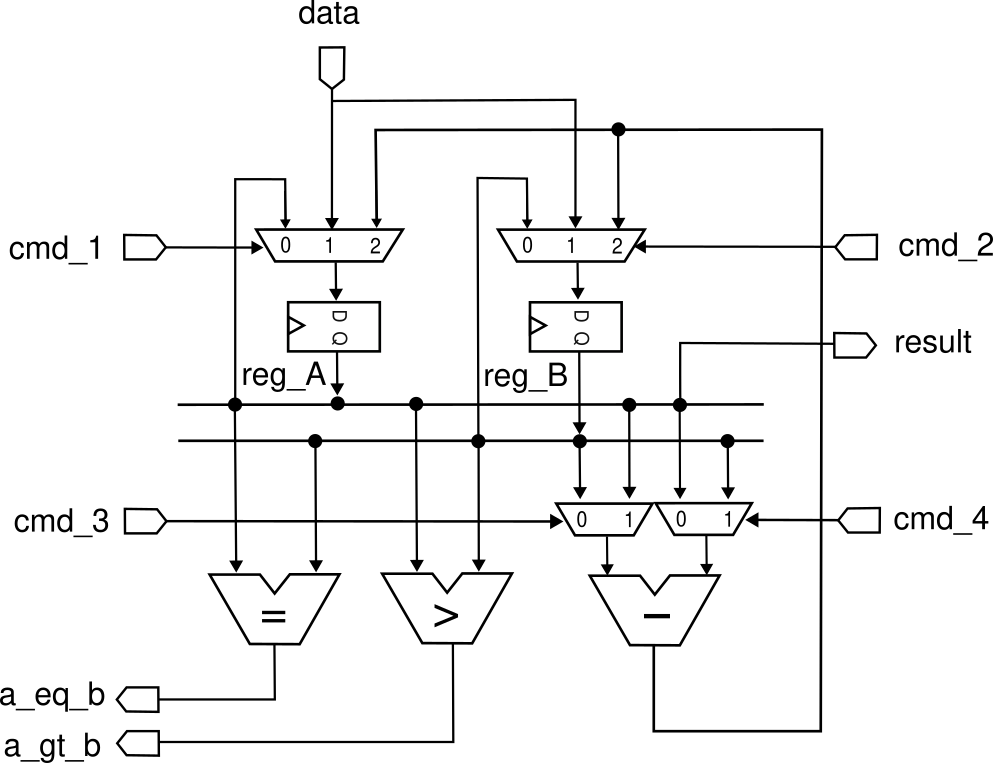
\includegraphics[scale=0.3]{./images/gcd_0}
      \end{center}
    \end{column}
  \end{columns}
\end{frame}

\begin{frame}[t]{Séquencement de $\mathrm{pgcd}(48,18)$ : }
  \centering
  \footnotesize
  \setlength{\tabcolsep}{5pt}
  \renewcommand{\arraystretch}{1.2}
  \begin{tabular}{@{}r l r c c c c r r l@{}}
    \toprule
    \textbf{Cycle} & \textbf{État} & \texttt{data} &
    \texttt{cmd\_1} & \texttt{cmd\_2} & \texttt{cmd\_3} & \texttt{cmd\_4} &
    \texttt{reg\_a} & \texttt{reg\_b} & \textbf{Action du datapath} \\
    \midrule
    0 & IDLE & -- & 0 & 0 & \textcolor{gray}{0} & \textcolor{gray}{0} & 0 & 0 & \texttt{go}=1 échantillonné \\
    1 & READ\_A & 48 & \cellcolor{hl}\textbf{1} & 0 & \textcolor{gray}{0} & \textcolor{gray}{0} & 0 & 0 & \texttt{reg\_a} $\leftarrow$ \texttt{data} \\
    2 & READ\_B & 18 & 0 & \cellcolor{hl}\textbf{1} & \textcolor{gray}{0} & \textcolor{gray}{0} & 48 & 0 & \texttt{reg\_b} $\leftarrow$ \texttt{data} \\
    3 & COMPUTE & -- & \cellcolor{hl}\textbf{2} & 0 & \cellcolor{hl}\textbf{0} & \cellcolor{hl}\textbf{1} & 48 & 18 & $a>b$ : $a \leftarrow a-b$ \\
    4 & COMPUTE & -- & \cellcolor{hl}\textbf{2} & 0 & \cellcolor{hl}\textbf{0} & \cellcolor{hl}\textbf{1} & 30 & 18 & $a>b$ : $a \leftarrow a-b$ \\
    5 & COMPUTE & -- & 0 & \cellcolor{hl}\textbf{2} & \cellcolor{hl}\textbf{1} & \cellcolor{hl}\textbf{0} & 12 & 18 & $a<b$ : $b \leftarrow b-a$ \\
    6 & COMPUTE & -- & \cellcolor{hl}\textbf{2} & 0 & \cellcolor{hl}\textbf{0} & \cellcolor{hl}\textbf{1} & 12 & 6 & $a>b$ : $a \leftarrow a-b$ \\
    7 & COMPUTE & -- & 0 & 0 & \textcolor{gray}{0} & \textcolor{gray}{0} & 6 & 6 & $a=b$ $\Rightarrow$ \texttt{done}=1 \\
    \bottomrule
  \end{tabular}

  \vspace{0.8em}
  \begin{minipage}{0.96\linewidth}
    \scriptsize
    \textbf{Lecture.}
    \texttt{cmd\_1}, \texttt{cmd\_2} : 0 = conserver, 1 = charger \texttt{data}, 2 = charger \texttt{computed\_value}.
    \texttt{cmd\_3}, \texttt{cmd\_4} : sélection des opérandes (0 = \texttt{reg\_a}, 1 = \texttt{reg\_b}), \texttt{computed\_value} = \texttt{arg\_1}$-$\texttt{arg\_2}.\\
    Les commandes sont décidées et appliquées dans le même cycle ; \texttt{reg\_x} est mis à jour au front de fin de cycle.
    \texttt{reg\_a} et \texttt{reg\_b} : valeurs au début du cycle. Une itération par cycle, \texttt{done} au cycle 7.
  \end{minipage}

\end{frame}

\begin{frame}{FSMD \texttt{GCD} : remarques}
  \textbf{Plusieurs remarques:}
  \begin{enumerate}
    \item Le choix retenu ici a été la \textbf{simplicité}.
    \begin{itemize}
      \item ...au détriment de la \textit{fréquence} de fonctionnement.
      \item Notamment, le \textit{chemin critique} est \textit{assez} long :
        \begin{itemize}
          \item Logique combinatoire FSM $\Rightarrow$ logique combinatoire sélection datapath.
        \end{itemize}
    \end{itemize}
   \item Ce chemin peut être réduit par des schémas d'interposition de registres entre FSM et datapath.
   \item Mais la mise au point est plus complexe :
     \begin{itemize}
      \item Actions déclanchées à un \textbf{cycle donné}...
      \item ...dont les effets s'effectuent au \textbf{cycle suivant}.
    \end{itemize}
    \item Pipelining complexe
    \begin{itemize}
      \item Peut nécessiter des \textbf{anticipations} (\texttt{forwarding})
      \item etc
    \end{itemize}
    \item \textbf{Note :} toute la démarche implique l'existence d'un \textit{protocole} d'utilisation du circuit. Notamment l'ordre de présentation des données devra être connu au moment de la conception et respecté au moment de l'utilisation.
    %\item Le PGCD ne présente pas de \textbf{dépendances de données} complexes (voir dernier TD).
  \end{enumerate}
\end{frame}
